\documentclass{standalone}
\usepackage{pgfplots}
\usepackage{amsmath}
\usepackage{amssymb}

\begin{document}
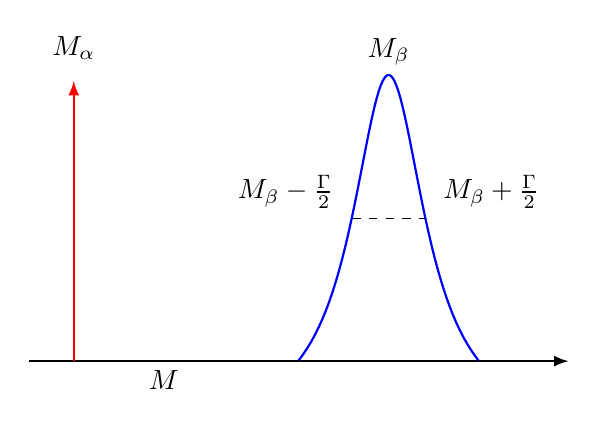
\begin{tikzpicture}
    \begin{axis}[
        domain=3:7, % Limitar la curva de la Lorenziana entre 3 y 7
        samples=100,
        axis lines=middle,
        axis x line=middle, % Solo el eje horizontal
        axis y line=none, % Eliminar el eje vertical
        axis line style={-latex, thick}, % Flecha al final del eje x
        tick style={draw=none}, % Sin tics
        xtick=\empty, % Sin números en el eje x
        ytick=\empty, % Sin números en el eje y
        xlabel style={draw=none}, % Ocultar la etiqueta del eje x
        xmin=-3, xmax=9, % Mostrar el eje desde -3 hasta 7
        ymin=-0.05, ymax=0.35 % Ajustar el rango en y para que el gráfico esté sobre el eje
    ]
    
    % Definición de la Lorenziana con gamma = 1 y centrada en x_0 = 5, solo visible entre x=3 y x=7
    \addplot[blue, thick, domain=3:7] {1/(pi) * 1 / ((x-5)^2 + 1) - 0.063};
    
    % Añadir una etiqueta en el pico (x=5, y=1/pi - 0.063)
    \node at (axis cs:5,0.255) [anchor=south] {$M_\beta$};

    % Delta de Dirac en x=-2, ajustada para descansar en el eje
    \draw[red, thick, -latex] (axis cs:-2,0) -- (axis cs:-2,0.25);
    \node at (axis cs:-2, 0.26) [anchor=south] {$M_\alpha$}; % Etiqueta M_\alpha

    % Etiqueta en x=0 ajustada sobre el eje
    \node at (axis cs:0, 0) [anchor=north] {$M$};

    % Añadir una línea horizontal en la mitad de la Lorenziana
    \draw[dashed] (axis cs:4.2, 0.1275) -- (axis cs:5.8, 0.1275); % Línea horizontal a la mitad del nuevo pico

    % Etiqueta en el extremo izquierdo de la línea horizontal
    \node at (axis cs:4, 0.1275) [anchor=south east] {$M_\beta - \frac{\Gamma}{2}$};

    % Etiqueta en el extremo derecho de la línea horizontal
    \node at (axis cs:6, 0.1275) [anchor=south west] {$M_\beta + \frac{\Gamma}{2}$};
    \end{axis}
\end{tikzpicture}
\end{document}
